\documentclass[11pt, a4paper, twoside]{article}
% Latex version of times new roman
%\usepackage{mathptmx}

\usepackage[utf8]{inputenc}
\usepackage[german, british]{babel}
\usepackage[useregional]{datetime2}
\usepackage[hcentering,bindingoffset=8mm,top=4cm,bottom=4cm,left=3cm,right=2.75cm,asymmetric, headheight=13.6pt]{geometry}
\usepackage{mathtools}

% frs direkte Verlinken des Inhaltsverzeichnisses und anderer Links
\usepackage{hyperref}
\hypersetup{pdfborder = {0 0 0}}

% zustzliche mathematische Symbole, AMS=American Mathematical Society 
\usepackage{amssymb}
\usepackage{bbm}

% frs Einbinden von Graphiken
\usepackage{graphicx}
\graphicspath{{./images/}}

\usepackage{caption}
\usepackage{subcaption}

% Tilde and other special characters
\usepackage{textcomp}

% Set the paragraph identation to 0
\setlength\parindent{0pt}

% Picture placement
\usepackage{float}

\usepackage[round, authoryear]{natbib}
\usepackage{array}

% colors
\usepackage{xcolor}
\usepackage{color}

% Code environment
\usepackage{listings}

% Package for enumerations
\usepackage{enumitem}

\definecolor{mygreen}{rgb}{0,0.7,0.3}

\lstdefinestyle{intaRNAOutput}{
	basicstyle={\ttfamily\small},
	keepspaces=true,
	moredelim=**[is][\color{mygreen}]{@}{@},
	moredelim=**[is][\color{blue}]{\$}{\$},
	moredelim=**[is][\color{red}]{\{}{\}}
}

\newcolumntype{L}[1]{>{\raggedright\let\newline\\\arraybackslash\hspace{0pt}}m{#1}}
\newcolumntype{C}[1]{>{\centering\let\newline\\\arraybackslash\hspace{0pt}}m{#1}}
\newcolumntype{R}[1]{>{\raggedleft\let\newline\\\arraybackslash\hspace{0pt}}m{#1}}

\newcommand{\univname}{Albert-Ludwigs University of Freiburg}
\newcommand{\ttitle}{Constrained RNA-RNA interaction prediction}
\newcommand{\sttitle}{}
\newcommand{\authorname}{Rick Gelhausen}
\newcommand{\supnames}{Dr. Martin Raden}
\newcommand{\fExaminer}{Prof. Dr. Rolf Backofen}
\newcommand{\sExaminer}{Prof. Ivo L. Hofacker}
\newcommand{\uniVienna}{University of Vienna}
\newcommand{\degreename}{Master of Science}
\newcommand{\groupname}{Bioinformatics Group}
\newcommand{\deptname}{Department of Computer Science}
\newcommand{\handindate}{\DTMdisplaydate{2018}{6}{1}{-1}} 

% Commands
% Variables
\newcommand{\seq}{S} % sequence
\newcommand{\str}{P} % structure
\newcommand{\ens}{\mathcal{\str}} % structure ensemble
\newcommand{\ensAll}{\ens_{\text{all}}} % ensemble of all structures
\newcommand{\en}{E} % Energy
\newcommand{\parr}{Z} % Partition function
\newcommand{\parrall}{\parr_{\ŧext{all}}} % partition function of ensemble of all structures
\newcommand{\parrun}{\parr_{i,j}^u} % partition function of unpaired region [i,j]
\newcommand{\nI}{n_{I}} % number of paired bases
\newcommand{\nP}{n_{B}} % number of interior unpaired bases
\newcommand{\altP}{B} % replacing P with new parameter to avoid confusion
% Special
\newcommand{\ubold}[1]{\underline{\textbf{#1}}}

% Helix functions
\newcommand{\helixSeed}{E_{helix}^{seed}}
\newcommand{\helix}{E_{helix}}

% seed function
\newcommand{\seed}{E_{seed}}
\newcommand{\HRule}{\rule{\linewidth}{0.5mm}}

% fr Namen etc. in Kopf- oder Fuzeile
\usepackage{fancyhdr}
% erlaubt benutzerdefinierte Kopfzeilen 
\pagestyle{fancy}
\newcolumntype{Y}{>{\raggedright\arraybackslash}X}
\fancypagestyle{abstract}
{
	\fancyhf{}
	\renewcommand\headrulewidth{0pt}
	\renewcommand\footrulewidth{0pt}
	\fancyfoot[C]{\thepage}
}
\newcommand*{\figuretitle}[1]{%
	{\centering
		\textbf{#1} 
		\par\medskip}
}
\fancypagestyle{plain}
{
	\fancyhf{}
	\renewcommand\headrulewidth{0pt}
	\renewcommand\footrulewidth{0pt}
	\fancyfoot[C]{Page \thepage}
}
\fancypagestyle{fancyp}{
	\fancyhf{}
	\renewcommand\headrulewidth{0.4pt}
	\fancyhead[R]{\sttitle}
	\fancyhead[C]{\textsc{\nouppercase{\leftmark}}}
	\fancyfoot[C]{Page \thepage}
}
\fancypagestyle{bibo}{
	\fancyhf{}
	\renewcommand\headrulewidth{0.4pt}
	\fancyhead[C]{\leftmark}
	\fancyfoot[C]{Page \thepage}
}
	
\renewcommand{\chaptermark}[1]{\markboth{\MakeUppercase{#1}}{}}

\begin{document}
	
	\pagenumbering{roman}
	
	\pagestyle{fancyp}
	\pagenumbering{arabic}
	\section{Recursions}

\subsection{Definitions}

$S^1, S^2$ target and query sequences\\
$i_1, j_1, i_2, j_2$ interaction boundaries\\
$si_1, sj_1, si_2, sj_2$ seed boundaries\\
$N$ the maximum interaction length $(\sim 150)$\\
$M$ the enclosed unpaired positions in one loop $(\sim 15)$

General energy computation:

\begin{figure}[H]
	\centering
	\includegraphics[scale=0.45]{seedenergy_general.png}
\end{figure}

\begin{equation*}
E(\substack{i_1,j_1\\i_2,j_2}) = E_{h}(\substack{i_1,j_1\\i_2,j_2}) + ED_{1}(\substack{i_1\\j_1}) + ED_{2}(\substack{i_2\\j_2})
\end{equation*}

Optimization task: [TODO]

\subsection{Initialization}

\begin{equation*}
\underset{{\substack{si_1 <= i_{1} <= j_{1} <= sj_{1}\\si_2 <= i_{2} <= j_{2} <= sj_{2}}}}{\forall} E_h(\substack{i_1,j_1\\i_2,j_2}) = \infty
\end{equation*}

\begin{equation*}
E_h(\substack{si_1,sj_1\\si_2,sj_2}) = E_{seed}
\end{equation*}

\clearpage

\subsection{Recursion 1 ($O(N^{4})$ space + time)}

\begin{figure}[H]
	\centering
	\includegraphics[scale=0.65]{seedenergy.png}
\end{figure}

\begin{equation*}
\substack{
  \underset{\substack{si_{1}-N <= i_{1} <= si_{1}\\si_{2}-N <= i_{2} <= si_{2}}}{\forall}\\
  \underset{\substack{sj_{1} <= j_{1} <= sj_{1}+N\\sj_{2} <= j_{2} <= sj_{2}+N}}{\forall}
}
E_h(\substack{i_1,j_1\\i_2,j_2}) = \begin{cases}
  \infty\\
  \quad\text{: if } \text{ no matching base pair }\\
  \infty\\
  \quad\text{: if } j_{1} - i_{1} > N \text{ oder } j_{2} - i_{2} > N\\
  \min\limits_{\substack{i_{1} < l_{1} <= r_{1} < j_{1}\\i_{2} < l_{2} <= r_{2} < j_{2}\\l_{1} - i_{1} - 1 <= M\\j_{1}-r_{1}-1 <= M\\l_{2} - i_{2} - 1 <= M\\j_{2}-r_{2}-1 <= M}}
  \begin{pmatrix}
	E_{loop}(\substack{i_1,l_1\\i_2,l_2}) + E_h(\substack{l_1,r_1\\l_2,r_2}) + E_{loop}(\substack{r_1,j_1\\r_2,j_2})
  \end{pmatrix}\\
  \quad\text{: otherwise.}\\
  
\end{cases}
\end{equation*}

\clearpage

\subsection{Recursion 2 ($O(N^{2})$ space + $O(N^{4})$ time)}

\begin{figure}[H]
	\centering
	\includegraphics[scale=0.65]{seedenergy2.png}
\end{figure}

\begin{equation*}
E_h(\substack{i_1,j_1\\i_2,j_2}) = \begin{cases}
\infty\\
\quad\text{: if } j_{1} - i_{1} > N \text{ oder } j_{2} - i_{2} > N\\
\begin{pmatrix}
E_{L}(\substack{i_1\\i_2}) + E_{seed} + E_{R}(\substack{j_1\\j_2})
\end{pmatrix}\\
\quad\text{: otherwise.}\\
\end{cases}
\end{equation*}

\begin{equation*}
\underset{\substack{si_{1}-N <= i_{1} <= si_{1}\\si_{2}-N <= i_{2} <= si_{2}}}{\forall}\\
E_L(\substack{i_1\\i_2}) = \begin{cases}
\infty\\
\quad\text{: if } \text{ no matching base pair }\\
\min\limits_{\substack{l_{1} - i_{1} - 1 <= M\\l_{2} - i_{2} - 1 <= M}}
\begin{pmatrix}
E_L(\substack{l_1\\l_2}) + E_{loop}(\substack{i_1,l_1\\i_2,l_2})
\end{pmatrix}\\
\quad\text{: otherwise.}\\

\end{cases}
\end{equation*}

\begin{equation*}
\underset{\substack{sj_{1} <= j_{1} <= sj_{1}+N\\sj_{2} <= j_{2} <= sj_{2}+N}}{\forall}
E_R(\substack{j_1\\j_2}) = \begin{cases}
\infty\\
\quad\text{: if } \text{ no matching base pair }\\
\min\limits_{\substack{j_{1}-r_{1}-1 <= M\\j_{2}-r_{2}-1 <= M}}
\begin{pmatrix}
E_{loop}(\substack{r_1,j_1\\r_2,j_2}) + E_R(\substack{r_1\\r_2})
\end{pmatrix}\\
\quad\text{: otherwise.}\\

\end{cases}
\end{equation*}


\end{document}